
% ----------------------------------------------------------------------
%  Set the document class
% ----------------------------------------------------------------------
\documentclass[11pt,a4paper,twoside]{article}

% ----------------------------------------------------------------------
% Define external packages, language, margins, fonts and new commands
% ----------------------------------------------------------------------
%\input{preamble} 
\usepackage[utf8]{inputenc}   % <<<<< Linux
\usepackage[english]{babel} % <<<<< English
\usepackage{notoccite}
\usepackage[skip=0.5\baselineskip]{caption}
\hyphenation{GTKWave}
\usepackage{listings}
\usepackage[all]{nowidow}

%blind text
\usepackage{lipsum}

\usepackage{graphicx}
\graphicspath{{./}{../../figlib/}{../mat/}{../sim/}}
\def\FontLn{% 16 pt normal
  \usefont{T1}{phv}{m}{n}\fontsize{16pt}{16pt}\selectfont}
\def\FontLb{% 16 pt bold
  \usefont{T1}{phv}{b}{n}\fontsize{16pt}{16pt}\selectfont}
\def\FontMn{% 14 pt normal
  \usefont{T1}{phv}{m}{n}\fontsize{14pt}{14pt}\selectfont}
\def\FontMb{% 14 pt bold
  \usefont{T1}{phv}{b}{n}\fontsize{14pt}{14pt}\selectfont}
\def\FontSn{% 12 pt normal
  \usefont{T1}{phv}{m}{n}\fontsize{12pt}{12pt}\selectfont}

% Use Arial font as default
%
\renewcommand{\rmdefault}{phv}
\renewcommand{\sfdefault}{phv}
\usepackage{geometry}	
\geometry{verbose,tmargin=2.5cm,bmargin=2.5cm,lmargin=2.5cm,rmargin=2.5cm}

%\usepackage{setspace}
%\renewcommand{\baselinestretch}{1.5}

\usepackage[pdftex]{hyperref} % enhance documents that are to be
                              % output as HTML and PDF
\hypersetup{colorlinks,       % color text of links and anchors,
                              % eliminates borders around links
%            linkcolor=red,    % color for normal internal links
            linkcolor=black,  % color for normal internal links
            anchorcolor=black,% color for anchor text
%            citecolor=green,  % color for bibliographical citations
            citecolor=black,  % color for bibliographical citations
%            filecolor=magenta,% color for URLs which open local files
            filecolor=black,  % color for URLs which open local files
%            menucolor=red,    % color for Acrobat menu items
            menucolor=black,  % color for Acrobat menu items
%            pagecolor=red,    % color for links to other pages
            pagecolor=black,  % color for links to other pages
%            urlcolor=cyan,    % color for linked URLs
            urlcolor=black,   % color for linked URLs
	          bookmarks=true,         % create PDF bookmarks
	          bookmarksopen=false,    % don't expand bookmarks
	          bookmarksnumbered=true, % number bookmarks
	          pdftitle={report},
            pdfauthor={Andre C. Marta},
%            pdfsubject={Thesis Title},
%            pdfkeywords={Thesis Keywords},
            pdfstartview=FitV,
            pdfdisplaydoctitle=true}

\usepackage[numbers,sort&compress]{natbib} % <<<<< References in numbered list [1],[2],...
\usepackage{subcaption} 
\usepackage{mdframed}

%%%%%%%%%%%%%%%%%%%%%%%%%%%%%%%%%%%%%%%%%%%%%%%%%%%%%%%%%%%%%%%%%%%%%%%%
%     Begin Document                                                   %
%%%%%%%%%%%%%%%%%%%%%%%%%%%%%%%%%%%%%%%%%%%%%%%%%%%%%%%%%%%%%%%%%%%%%%%%


\begin{document}

% Set plain page style (no headers, footer with centered page number)
\pagestyle{plain}

% Set roman numbering (i,ii,...) before the start of chapters
%\pagenumbering{roman}

% ----------------------------------------------------------------------
%  Cover page
% ----------------------------------------------------------------------
%%%%%%%%%%%%%%%%%%%%%%%%%%%%%%%%%%%%%%%%%%%%%%%%%%%%%%%%%%%%%%%%%%%%%%%%
%                                                                      %
%     File: Thesis_FrontCover.tex                                      %
%     Tex Master: Thesis.tex                                           %
%                                                                      %
%     Author: Andre C. Marta                                           %
%     Last modified :  2 Jul 2015                                      %
%                                                                      %
%%%%%%%%%%%%%%%%%%%%%%%%%%%%%%%%%%%%%%%%%%%%%%%%%%%%%%%%%%%%%%%%%%%%%%%%

\thispagestyle {empty}

% IST Logo - Signature A
% parameters: bb=llx lly urx ury (bounding box), width=h_length, height=v_length, angle=angle, scale=factor, clip=true/false, draft=true/false. 
\includegraphics[bb=9.5cm 11cm 0cm 0cm,scale=0.29]{IST_A_CMYK_POS}

\begin{center}
%
% Figure (Image or plot)
\vspace{1.0cm}
% height = 50 mm
%\includegraphics[height=50mm]{Figures/Airbus_A350.jpg}

% Title, author and degree
\vspace{1cm}
{\FontLb Circuit Theory and Electronics Fundamentals} \\ % <<<<< EDIT TITLE
\vspace{1cm}
{\FontSn Técnico, University of Lisbon} \\ % <<<<< EDIT COURSE
\vspace{1cm}

{\FontSn T5: Bandpass filter using OP-AMP} \\
\vspace{1cm}
{\FontSn Diogo Pereira, n.º95780}
%\vspace{0.5cm}
\par{\FontSn Manuel Braga, n.º95821}
%\vspace{0.5cm}
\par{\FontSn Pedro Silva, n.º95839}
\vspace{1.0cm}
\par{\FontSn June 6, 2021} \\ % <<<<< EDIT DATE (corresponds to date of oral examination)
%
\end{center}



% ----------------------------------------------------------------------
% Dedication page (optional)
% ----------------------------------------------------------------------
%\input{dedication} 
%\cleardoublepage

% ----------------------------------------------------------------------
%  Acknowledgments (optional)
% ----------------------------------------------------------------------
%\input{acknowledgements}
%\cleardoublepage

% ----------------------------------------------------------------------
%  Abstract (both in English and Portuguese)
% ----------------------------------------------------------------------
%\input{resumo} 
%\cleardoublepage

%\input{abstract} 

% ----------------------------------------------------------------------
%  Table of contents, list of tables, list of figures and nomenclature
% ----------------------------------------------------------------------

% Table of contents
%
\tableofcontents

% List of tables
%\addcontentsline{toc}{section}{\listtablename}
%\listoftables
%\cleardoublepage 

% List of figures
%\addcontentsline{toc}{section}{\listfigurename}
%\listoffigures
%\cleardoublepage 

% Set arabic numbering (1,2,...) after preface
%
%\setcounter{page}{1}
%\pagenumbering{arabic}

% ----------------------------------------------------------------------
%  Body
% ----------------------------------------------------------------------

\section{Introduction}
\label{sec:introduction}

% state the learning objective 

\par The objective of this laboratory assignment is to study an RC circuit as described in Figure~\ref{fig:rc}.


\begin{figure}[h]
\centering
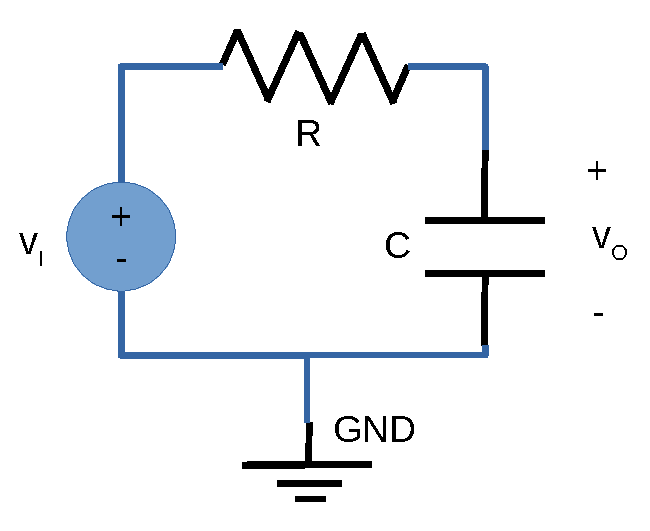
\includegraphics[width=0.9\linewidth]{../doc/rc.pdf}
\caption{T2 RC circuit.}
\label{fig:rc}
\end{figure}


\par In Section~\ref{sec:analysis}, a theoretical analysis of the circuit is made, by applying different methods, such as the Thevenin and Phasor analysis, and the total solution (natural plus forced solutions) of the circuit is presented. The theoretical frequency response of the circuit is also presented in this section. In Section~\ref{sec:simulation}, the circuit is analysed by simulation in NGSpice and the results obtained for the operating point and transient analysis are compared to the theoretical results obtained in Section~\ref{sec:analysis}. The conclusions of this study are outlined in Section~\ref{sec:conclusion}.

$NOTE:$~This report was automatically generated. The data used was supplied by inputting 95780 to the $t2\_datagen.py$ file. A different set of data should automatically yield coherent results.



\section{Theoretical Analysis}
\label{sec:analysis}

In this section, the circuit shown in Figure~\ref{fig:rc} is analysed
theoretically, in terms of the voltages and current intensities in the various branches and components of the circuit.

For convenience and coherence purposes, we chose to number the nodes of this circuit in the same manner that they will be numbered in the modified circuit used in the simulation. This means that nodes with the same number are in equivalent positions in the two circuits and explains why some numbers are skipped in this original circuit (the modified circuit has more nodes). In section ----- these modifications will be properly explained.

\subsection{Mesh Method}

The circuit consists of multiple loops with various values of current, $i$, circulating in each of the branches of the circuit. There are two
voltage sources, $v_a$ and $v_c$, driving their inputs. Applying the Mesh Method, we reach a system of 5 equations and 5 unkowns, that was solved with the aid of the Octave math tools. In ordersystem into a matrix. Those equations are:

\begin{equation}
  mesh a -> v_a - R_1*i_a - R_3*(i_a + i_b) - R_4*(i_a +i_c) = 0.
\end{equation}

\begin{equation}
  mesh c -> v_c - R_4*(i_a +i_c) - (R_6 +R_7)*i_c = 0.
\end{equation}

Additional equations:
$v_c = K_c*i_c$
$i_b = K_b*v_b$
$v_b = R_3*(i_a + i_b)$

\subsection{Nodal Method}

Another way of solving the circuit is the Nodal Method, in which we have reached a system of 11 equations and 11 unknowns. After obtaining the equations, we repeated the procedure we took with the Mesh Method and solved the system with Octave software. The equations obtained by this method are:

\begin{equation}
  node 1 -> (v_2 - v_3)*G_1 + i_c +(v_1 - v_5)*G_4 = 0
\end{equation}

\begin{equation}
  node 3 -> (v_3 - v_5)*G_3 + (v_3 - v_2)*G_1 + (v_3 - v_4)*G_2 = 0.
  \label{eq:kvl}
\end{equation}

\begin{equation}
  node 4 -> (v_4 - v_3)*G_2 - i_b = 0.
\end{equation}

\begin{equation}
  node 6 -> i_b - i_d + (v_6 - v_5)*G_5 = 0.
  \label{eq:kvl2}
\end{equation}

Additional equations:
$v_1= 0$
$v_2 - v_1 = v_a$
$v_3 - v_5 = v_b$
$v_5 - v_9 = v_c$
$i_b = K_b*v_b$
$v_c = K_c*I_c$
$v_9 - v_1 = -i_c*(r_6 + r_7)$

Equation~(\ref{eq:kvl2}) 

The solution is of the form given in Equation~(\ref{eq:vo_for}) and is
illustrated in Figure~\ref{fig:forced}.





\begin{table}[h]
  \centering
  \begin{tabular}{|l|r|}
    \hline    
    {\bf Name} & {\bf Value [A or V]} \\ \hline
    Ia & 2.667112036144088e-01\\ \hline
Ib & -2.797307053897956e-01\\ \hline
Ic & 9.115165062107574e-01\\ \hline
Vb & -3.981339474096013e-02\\ \hline
Vc & 7.619521032756115\\ \hline

  \end{tabular}
  \caption{Table with the values of the unknowns from the system of equations obtained with the Mesh Method, solved using Octave; currents are expressed in Ampere and voltages are expressed Volts.}
  \label{tab:op}
\end{table}

\begin{table}[h]
  \centering
  \begin{tabular}{|l|r|}
    \hline    
    {\bf Name} & {\bf Value [A or V]} \\ \hline
    V0 & 0\\ \hline
V2 & 5.064003203930000\\ \hline
V3 & 4.796768408845987\\ \hline
V4 & 4.214279780392698\\ \hline
V5 & 4.836581803586947\\ \hline
V6 & 8.782125497855164\\ \hline
V9 & -2.782939229169170\\ \hline
Ib & -2.797307053897955e-01\\ \hline
Ic & 9.115165062107577e-01\\ \hline
Vb & -3.981339474096013e-02\\ \hline
Vc & 7.619521032756118\\ \hline

  \end{tabular}
  \caption{Table with the values of the unknowns from the system of equations obtained with the Nodal Method, solved using Octave; currents are expressed in Ampere and voltages are expressed Volts.}
  \label{tab:op}
\end{table}




\begin{equation}
  
  \label{eq:vo_for}
\end{equation}

\begin{figure}[h] \centering
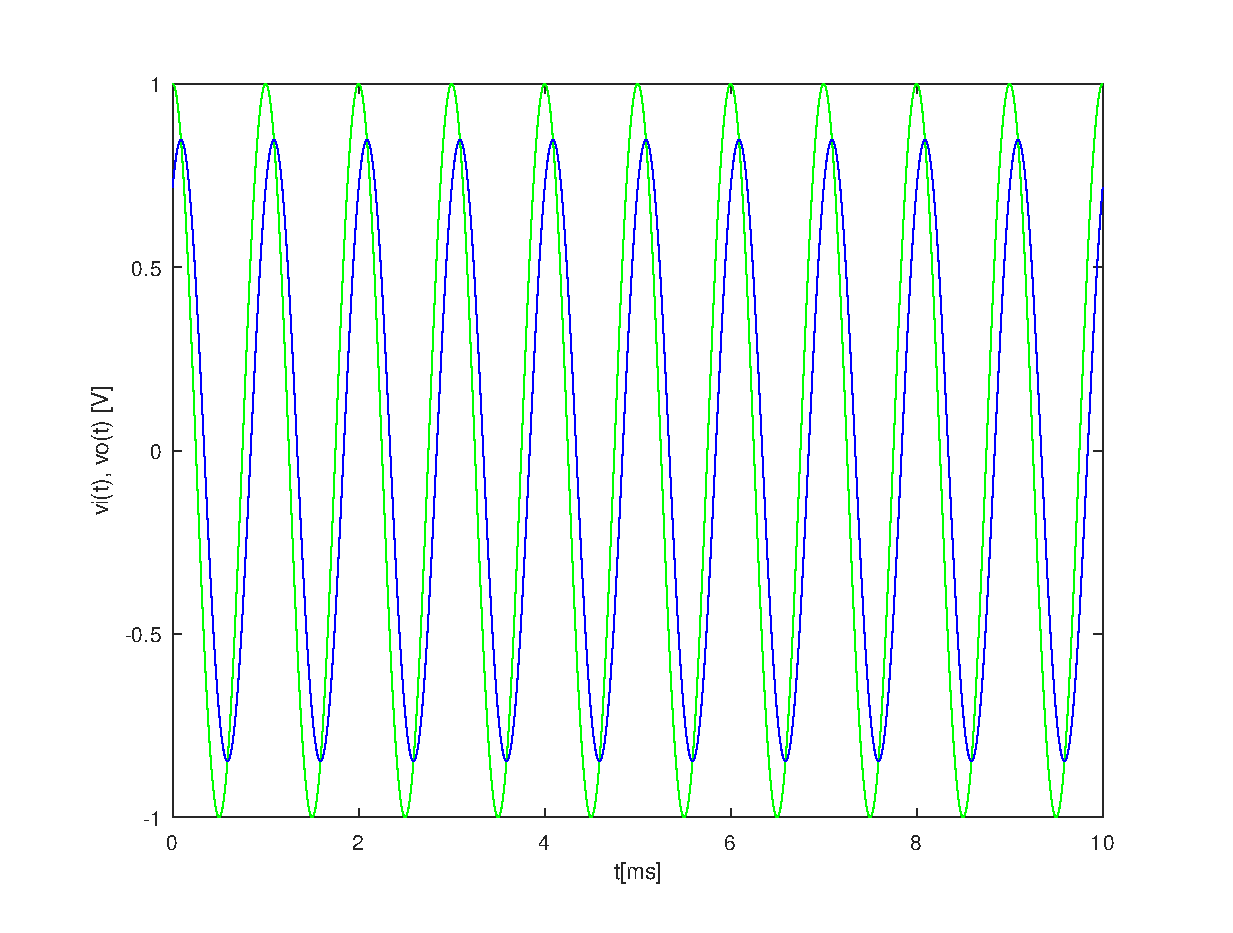
\includegraphics[width=0.8\linewidth]{forced.eps}
\caption{------------}
\label{fig:forced}
\end{figure}


\section{Simulation Analysis}
\label{sec:simulation}
Because the input voltage source in the circuit is sinusoidal, there is a variation in time in the voltage and current values of the various components. Therefore, it is important to analyse how they evolve in time and to picture the transformation of the AC input voltage source from the input to the output of this circuit. A transient analysis will be made, which helps in measuring the input and output impedance. The frequency response analysis will be made as well, so that the gain and central frequency of our output amplified sinusoidal signal can be determined.

\subsection{Frequency response and impedances}

The input and output impedances of the circuit are measured, the firstseen from the source's perspective, and the later seen from the output's perspective. With the frequency response, the voltage gain in the output and the lower and upper cut-off frequencies are measured. Using the same equation from the theoretical analysis the central frequency was determined, then extracting the output gain for such frequency. In Table~\ref{tab:main}, the results of the calculations are presented. In figures~\ref{fig:gainstage}and~\ref{fig:outputstage} the frequency response for our output's gain and phase, respectively, can be seen. In these figures a slightly narrow band-pass filter can be noticed. Regarding the phase plot, a full circle phase drop is noticed, until it reaches the $\ang{90}$ back again, unlike what happened in the theoretical analysis, in which the phase drops from $\ang{90}$ to $\ang{-90}$, where it stabilizes. This difference is the cause of the aproximation that is utilized to study the OP-AMP behaviour in the theoretical section. It was considered the OP-AMP did not introduce any phase difference in its output compared to its input, which is, in reality, not true. The transfer function in this sector actually presents 2 poles, which causes a double phase drop of $\ang{90}$ ($\ang{45}$ the decade before and $\ang{45}$ the decade after) each, which then means the phase actually drops $\ang{180}$ due to the OP-AMP, hence stabilizing not in $\ang{-90}$, but in $\ang{90}$ ($\ang{-270}$).

\begin{table}[h]
  \centering
  \begin{tabular}{|l|r|}
    \hline    
    {\bf Name} & {\bf Values} \\ \hline
    R1 & 1.00196314014\\ \hline 
R2 & 2.082319235\\ \hline
R3 & 3.05798143645\\ \hline
R4 & 4.10496355098\\ \hline 
R5 & 3.03658050119\\ \hline
R6 & 2.00356698935\\ \hline
R7 & 1.0495200477\\ \hline
Va & 5.06400320393\\ \hline
Id & 1.01960705059\\ \hline
Kb & 7.0260450587\\ \hline
Kc & 8.35916956066\\ \hline

    \input{outimp_tab}     
  \end{tabular}
  \caption{Center frequency, output gain and input and output impedances of the OP-AMP band-pass filter.}
  \label{tab:main}
\end{table}

The input impedance value is quite high. Therefore, depending on the input signal's inner resistance, it allows the majority of the input voltage to flow towards the OP-AMP. Consequently, the output impedance value is also quite high, which is not desirable. Therefore, for loads with low resistance values, most of the voltage will be consumed by the circuit's output impedance, which goes against what it was supposed to do. This band-pass filter is, then, more suited for loads with bigger values of resistance. 
Relatively to the obtained values for the central frequency and the gain for such frequency, there were slight deviations from the targeted values. A relative error of 1.863\% was obtained for the central frequency value, and 0.264\% for the output voltage gain, which we are good results.

\begin{figure}[h!] \centering
\includegraphics[width=0.6\linewidth]{vo1f.pdf}
\caption{Output voltage gain.}
\label{fig:gainstage}
\end{figure}

\begin{figure}[h!] \centering
\includegraphics[width=0.6\linewidth]{vo1p.pdf}
\caption{Output voltage phase difference.}
\label{fig:outputstage}
\end{figure}

\pagebreak
\subsection{Final result and merit}
The input and output signals can be compared, as seen in Figure~\ref{fig:comp}. The output voltage doesn't show a DC component, as expected. The evolution from the starting 10mV to the final (approximately) 1V amplitude is a direct result of the desired 40 dB gain, which corresponds to about 100 times the initial amplitude of the signal. In the first few milisseconds, a small variation in the output sinusoidal wave is seen, due to a small transient regime.


\begin{figure}[h!] \centering
\includegraphics[width=0.5\linewidth]{vo1.pdf}
\caption{Comparison between the input and the output sinusoidal signals.}
\label{fig:comp}
\end{figure}

\pagebreak

The cost and merit of our circuit are presented in Table~\ref{tab:merit}. As previously explained, the simulated central frequency and gain  were very close to the desired values, which results in very low relative errors, which imply small deviations. The overall cost of the circuit is high; however, it is primarily affected by the high cost of the OP-AMP subcircuit, which was unchangeable. The flipside of this was that using higher cost components in the rest of the circuit had less of an impact in the overall cost of the circuit as a whole. Because of this, the three $100 k\Omega$ resistors available in the amplification stage were utilized, which contributed to a close to perfect gain for the central frequency, without compromising the figure of merit. This figure is, in absolute terms, a very low number, however, we believe that, based on the restraints of the merit formula itself, it is an acceptable value.
\pagebreak

\par
\begin{table}[h!]
  \centering
  \begin{tabular}{|l|r|}
    \hline    
    {\bf Name} & {\bf Values} \\ \hline
    \input{merit_tab} 
  \end{tabular}
  \caption{Cost and merit.}
  \label{tab:merit}
\end{table}

\pagebreak


\section{Conclusion}
\label{sec:conclusion}

We achieved the goal of analyzing the given circuit for this laboratory assignment. We've performed both a theoretical analysis using Octave and a circuit simulation using Ngspice. The values given by the simulation were coincident with the ones that we got from the theoretical results. As this is a fairly simple circuit without any non-linear components, this result was expected.

%\cleardoublepage

% ----------------------------------------------------------------------
%  Bibliography
% ----------------------------------------------------------------------
%\addcontentsline{toc}{section}{\bibname}
%\bibliographystyle{abbrvunsrtnat} % <<<<< SELECT IF USING REFERENCES BY NUMBER (CITATION ORDER)
%\bibliography{../../../BIBfile.bib}

% ----------------------------------------------------------------------
\end{document}
% ----------------------------------------------------------------------
